\documentclass[notitlepage,a4paper]{article}\usepackage[]{graphicx}\usepackage[]{color}
%% maxwidth is the original width if it is less than linewidth
%% otherwise use linewidth (to make sure the graphics do not exceed the margin)
\makeatletter
\def\maxwidth{ %
  \ifdim\Gin@nat@width>\linewidth
    \linewidth
  \else
    \Gin@nat@width
  \fi
}
\makeatother

\definecolor{fgcolor}{rgb}{0.345, 0.345, 0.345}
\newcommand{\hlnum}[1]{\textcolor[rgb]{0.686,0.059,0.569}{#1}}%
\newcommand{\hlstr}[1]{\textcolor[rgb]{0.192,0.494,0.8}{#1}}%
\newcommand{\hlcom}[1]{\textcolor[rgb]{0.678,0.584,0.686}{\textit{#1}}}%
\newcommand{\hlopt}[1]{\textcolor[rgb]{0,0,0}{#1}}%
\newcommand{\hlstd}[1]{\textcolor[rgb]{0.345,0.345,0.345}{#1}}%
\newcommand{\hlkwa}[1]{\textcolor[rgb]{0.161,0.373,0.58}{\textbf{#1}}}%
\newcommand{\hlkwb}[1]{\textcolor[rgb]{0.69,0.353,0.396}{#1}}%
\newcommand{\hlkwc}[1]{\textcolor[rgb]{0.333,0.667,0.333}{#1}}%
\newcommand{\hlkwd}[1]{\textcolor[rgb]{0.737,0.353,0.396}{\textbf{#1}}}%
\let\hlipl\hlkwb

\usepackage{framed}
\makeatletter
\newenvironment{kframe}{%
 \def\at@end@of@kframe{}%
 \ifinner\ifhmode%
  \def\at@end@of@kframe{\end{minipage}}%
  \begin{minipage}{\columnwidth}%
 \fi\fi%
 \def\FrameCommand##1{\hskip\@totalleftmargin \hskip-\fboxsep
 \colorbox{shadecolor}{##1}\hskip-\fboxsep
     % There is no \\@totalrightmargin, so:
     \hskip-\linewidth \hskip-\@totalleftmargin \hskip\columnwidth}%
 \MakeFramed {\advance\hsize-\width
   \@totalleftmargin\z@ \linewidth\hsize
   \@setminipage}}%
 {\par\unskip\endMakeFramed%
 \at@end@of@kframe}
\makeatother

\definecolor{shadecolor}{rgb}{.97, .97, .97}
\definecolor{messagecolor}{rgb}{0, 0, 0}
\definecolor{warningcolor}{rgb}{1, 0, 1}
\definecolor{errorcolor}{rgb}{1, 0, 0}
\newenvironment{knitrout}{}{} % an empty environment to be redefined in TeX

\usepackage{alltt}
\usepackage[utf8]{inputenc}
\usepackage{pmboxdraw}
\usepackage[left=2.3cm,right=1.3cm,top=1.8cm]{geometry}
\usepackage{pdflscape}
\usepackage{anyfontsize}
\usepackage[smallscripts]{moresize}
\usepackage[a4paper,colorlinks]{hyperref}
\hypersetup{
    pdftitle = {State of the Art: PacBio Repeats},
    pdfsubject = {},
    pdfauthor = {Thierry Schuepbach}
}
\title{State of the Art\\ PacBio repeats through tweaked PfTools software suite}
\author{Thierry Schuepbach}
\IfFileExists{upquote.sty}{\usepackage{upquote}}{}
\begin{document}
\maketitle
\tableofcontents

\section{Description of the experiment}
In an attempt to account tandem repeats inside PacBio Next Generation Sequencing Technology data was generated for a single fixed number of repeat (to be determined) of "CAG" trinucleotides.\\
Available data files are:
\small{
\begin{verbatim}
├── [4.0K]  Analysis_Results
│   ├── [3.2G]  m160726_161412_42182_c101000162550000001823232709161623_s1_p0.1.bax.h5
│   ├── [448K]  m160726_161412_42182_c101000162550000001823232709161623_s1_p0.1.log
│   ├── [ 20M]  m160726_161412_42182_c101000162550000001823232709161623_s1_p0.1.subreads.fasta
│   ├── [ 40M]  m160726_161412_42182_c101000162550000001823232709161623_s1_p0.1.subreads.fastq
│   ├── [2.8G]  m160726_161412_42182_c101000162550000001823232709161623_s1_p0.2.bax.h5
│   ├── [442K]  m160726_161412_42182_c101000162550000001823232709161623_s1_p0.2.log
│   ├── [ 19M]  m160726_161412_42182_c101000162550000001823232709161623_s1_p0.2.subreads.fasta
│   ├── [ 37M]  m160726_161412_42182_c101000162550000001823232709161623_s1_p0.2.subreads.fastq
│   ├── [3.2G]  m160726_161412_42182_c101000162550000001823232709161623_s1_p0.3.bax.h5
│   ├── [440K]  m160726_161412_42182_c101000162550000001823232709161623_s1_p0.3.log
│   ├── [ 22M]  m160726_161412_42182_c101000162550000001823232709161623_s1_p0.3.subreads.fasta
│   ├── [ 43M]  m160726_161412_42182_c101000162550000001823232709161623_s1_p0.3.subreads.fastq
│   ├── [1.3M]  m160726_161412_42182_c101000162550000001823232709161623_s1_p0.bas.h5
│   ├── [ 74M]  m160726_161412_42182_c101000162550000001823232709161623_s1_p0.sts.csv
│   └── [128K]  m160726_161412_42182_c101000162550000001823232709161623_s1_p0.sts.xml
├── [220G]  m160726_161412_42182_c101000162550000001823232709161623_s1_p0.1.trx.h5
├── [8.8K]  m160726_161412_42182_c101000162550000001823232709161623_s1_p0.1.xfer.xml
├── [220G]  m160726_161412_42182_c101000162550000001823232709161623_s1_p0.2.trx.h5
├── [5.2K]  m160726_161412_42182_c101000162550000001823232709161623_s1_p0.2.xfer.xml
├── [220G]  m160726_161412_42182_c101000162550000001823232709161623_s1_p0.3.trx.h5
├── [5.2K]  m160726_161412_42182_c101000162550000001823232709161623_s1_p0.3.xfer.xml
├── [673M]  m160726_161412_42182_c101000162550000001823232709161623_s1_p0.mcd.h5
├── [3.9K]  m160726_161412_42182_c101000162550000001823232709161623_s1_p0.metadata.xml
└── [1.3M]  m160726_161412_42182_c101000162550000001823232709161623_s1_p0.trc.h5
\end{verbatim}
}
\section{Early methods and new addons to the PfTools}
\subsection{Perl scripts}
The following Perl script is used to account the number of "CAG" found within a subread:
\begin{verbatim}
cat xxx.fastq | perl -ne '@A=$_=~/(C{1,3}A{1,3}G{1,3})/g; printf "%d\n",$#A+1'
\end{verbatim}


\subsection{Addons to the PfTools: PfRepeat}
The PfTools suite as of version 3.x no longer had support for cyclic profiles. That feature was deprecated at the time of reimplementation in C due to the lack of use as opposed to the work involved.
I thus forked the code into a brand new tool "PfRepeat", reimplementing the connection so that input sequences could loop again on the profile if proven benefical.
Furthermore, several new analysis were added to fit the experiment goal, it is worth mentioning that unlike the Perl script, the code here always compute the reverse complement and chooses the best value.
\begin{enumerate}
  \item[Histogram] Given the number of bins, a histogram is generated for all subreads. That can be on the number of profile cycle or 
  \item[Density] Density plots are available to compare profile scores with profile number of cyles.
  \item[Standard regex] Regex sequences can be directly given instead or with a profile in order to account the number of matches.
  \item[Appended regex] As en extension to the previous analysis, we self-concatenate the regex sequence until nothing is found within the input string sequence. 
\end{enumerate}

PacBio pipeline exports sequences in FASTA format which is fine for the PfTools. Nevertheless, such available sequences have been filtered (quality, number of subreads, etc...). Therefore direct reading of PacBio native format was implemented to allow analysis not only on a subread basis but also on a hole basis. Output formats were modified accordingly to export interesting pieces of informations such as hole locations, qualities, types and number of subreads. At last, hole analysis would not be complete without mininum, maximum and mean computed values with respect to the number of subreads.



\section{Results so far}



\begin{knitrout}
\definecolor{shadecolor}{rgb}{0.969, 0.969, 0.969}\color{fgcolor}
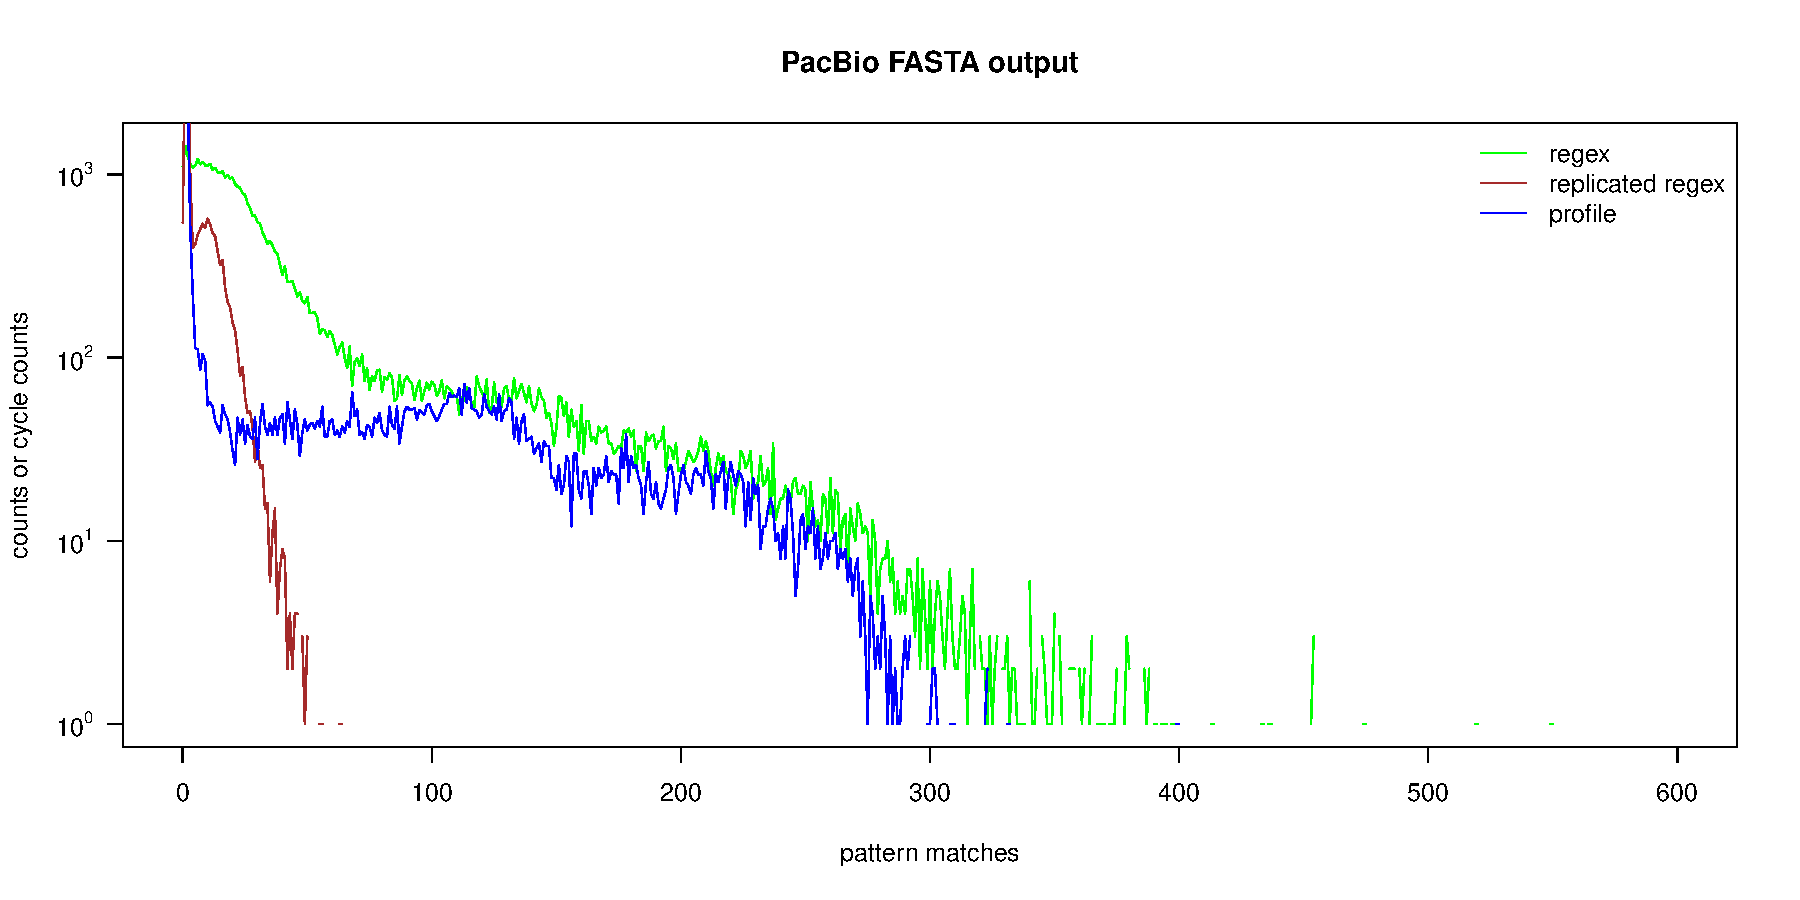
\includegraphics[width=\maxwidth]{figure/unnamed-chunk-2-1} 

\end{knitrout}

\begin{knitrout}
\definecolor{shadecolor}{rgb}{0.969, 0.969, 0.969}\color{fgcolor}
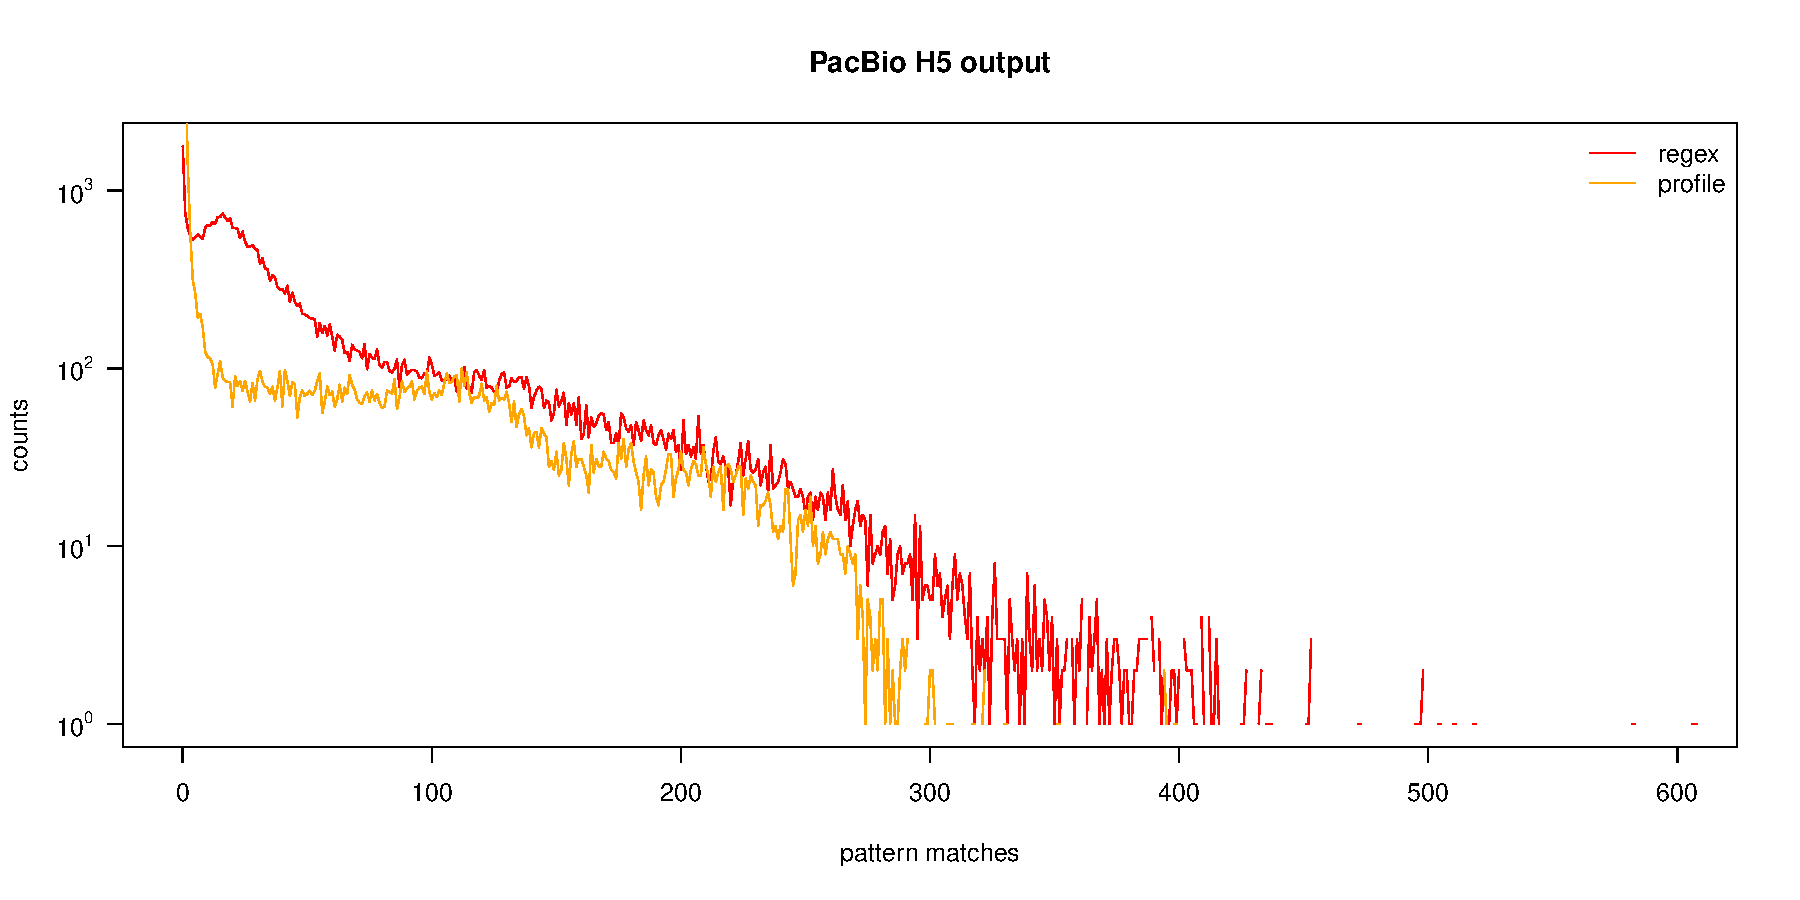
\includegraphics[width=\maxwidth]{figure/unnamed-chunk-3-1} 

\end{knitrout}

\begin{knitrout}
\definecolor{shadecolor}{rgb}{0.969, 0.969, 0.969}\color{fgcolor}
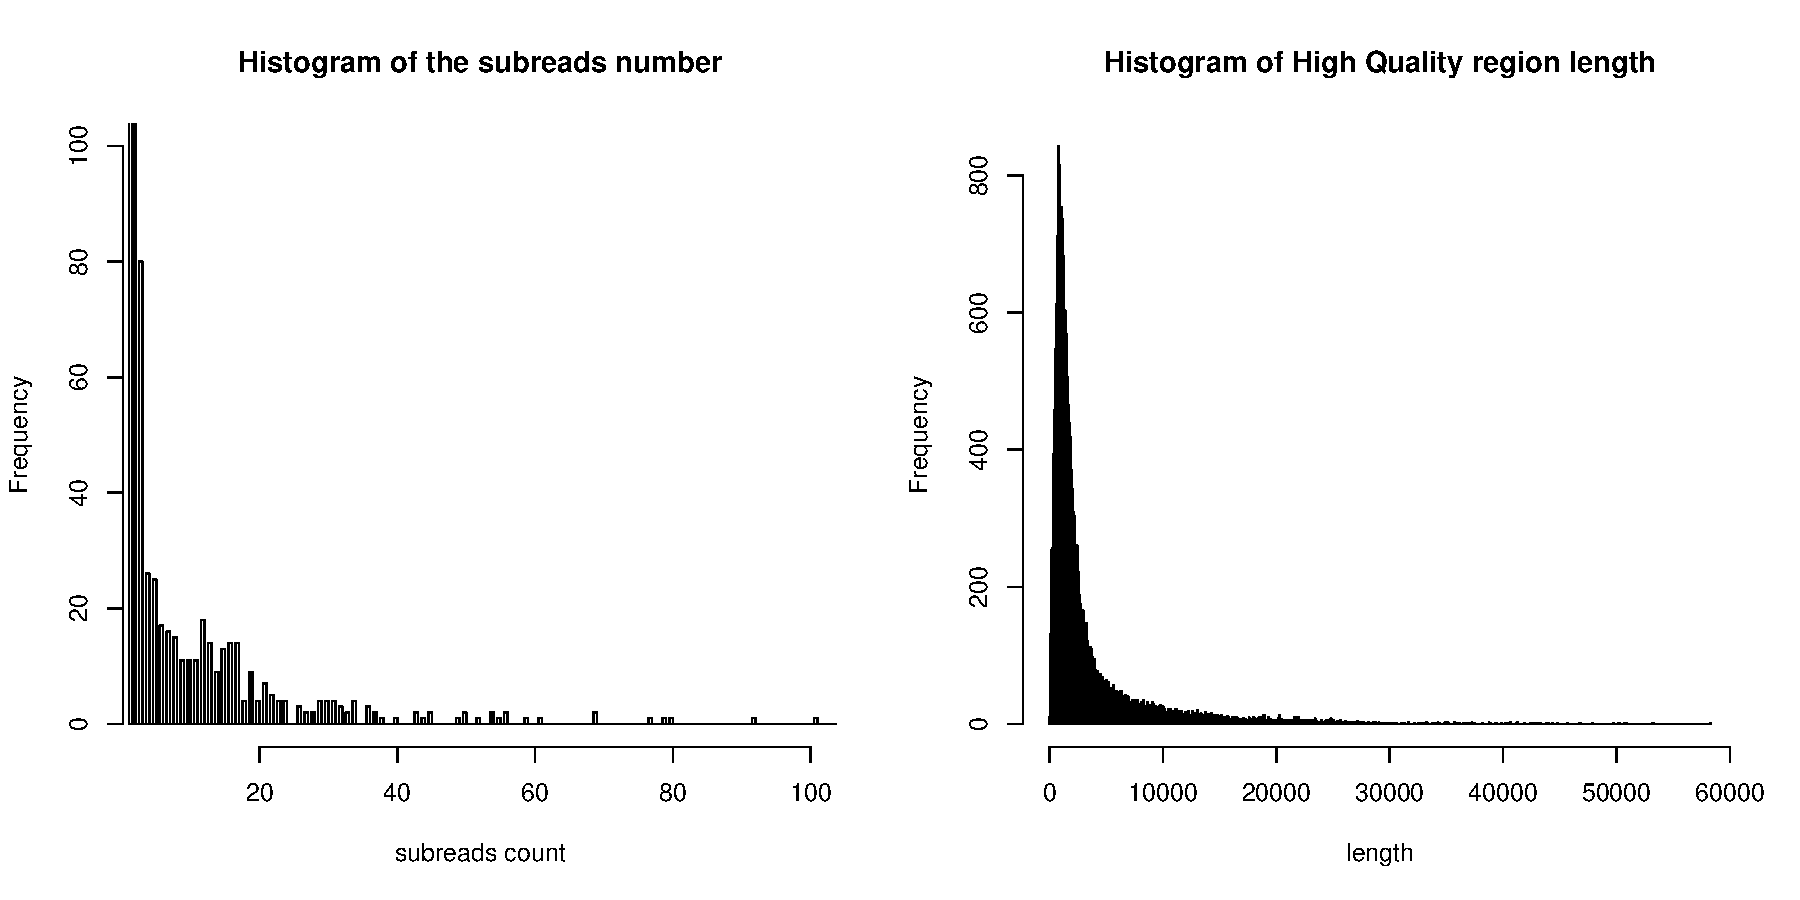
\includegraphics[width=\maxwidth]{figure/unnamed-chunk-4-1} 

\end{knitrout}

Carefully read the histogram plot of subreads number as it only shows the range $[4,100]$. 

\begin{knitrout}
\definecolor{shadecolor}{rgb}{0.969, 0.969, 0.969}\color{fgcolor}
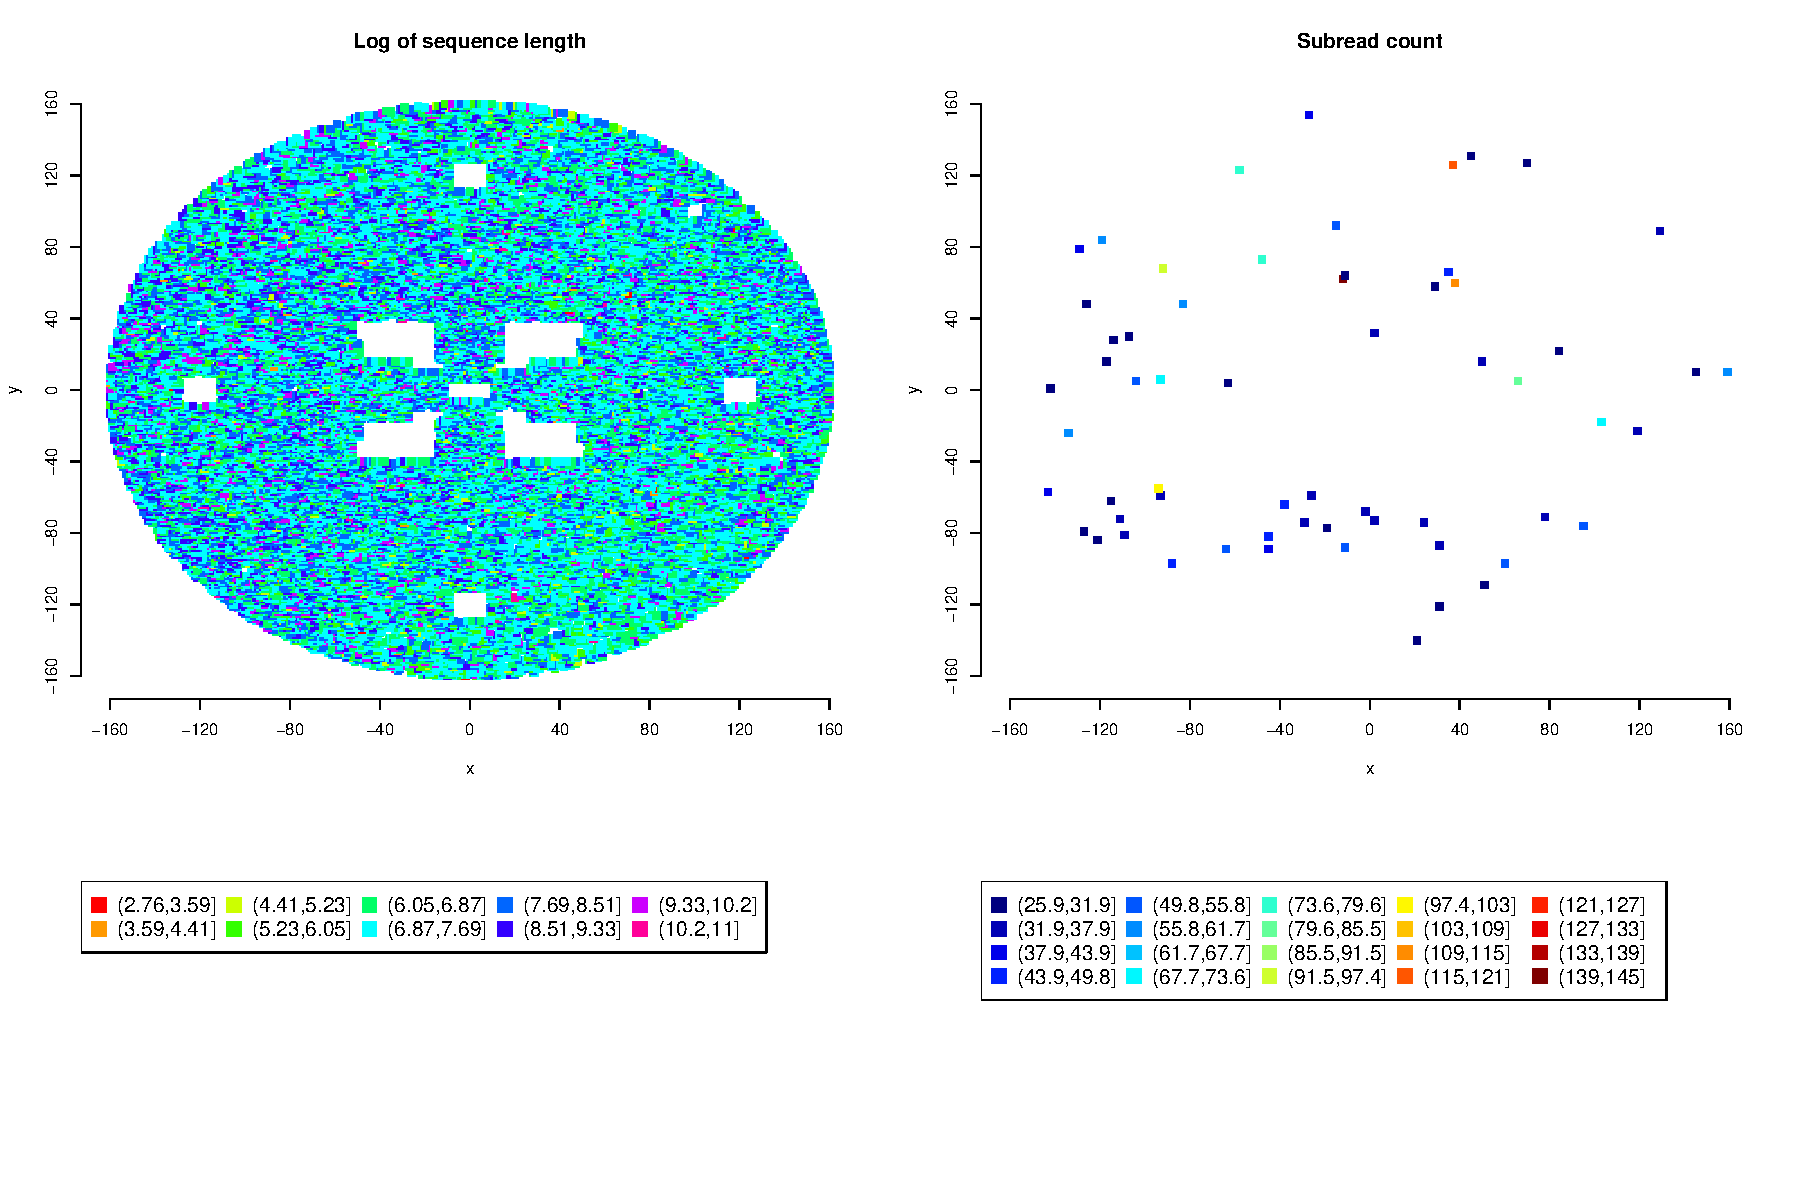
\includegraphics[width=\maxwidth]{figure/unnamed-chunk-5-1} 

\end{knitrout}

\begin{knitrout}
\definecolor{shadecolor}{rgb}{0.969, 0.969, 0.969}\color{fgcolor}
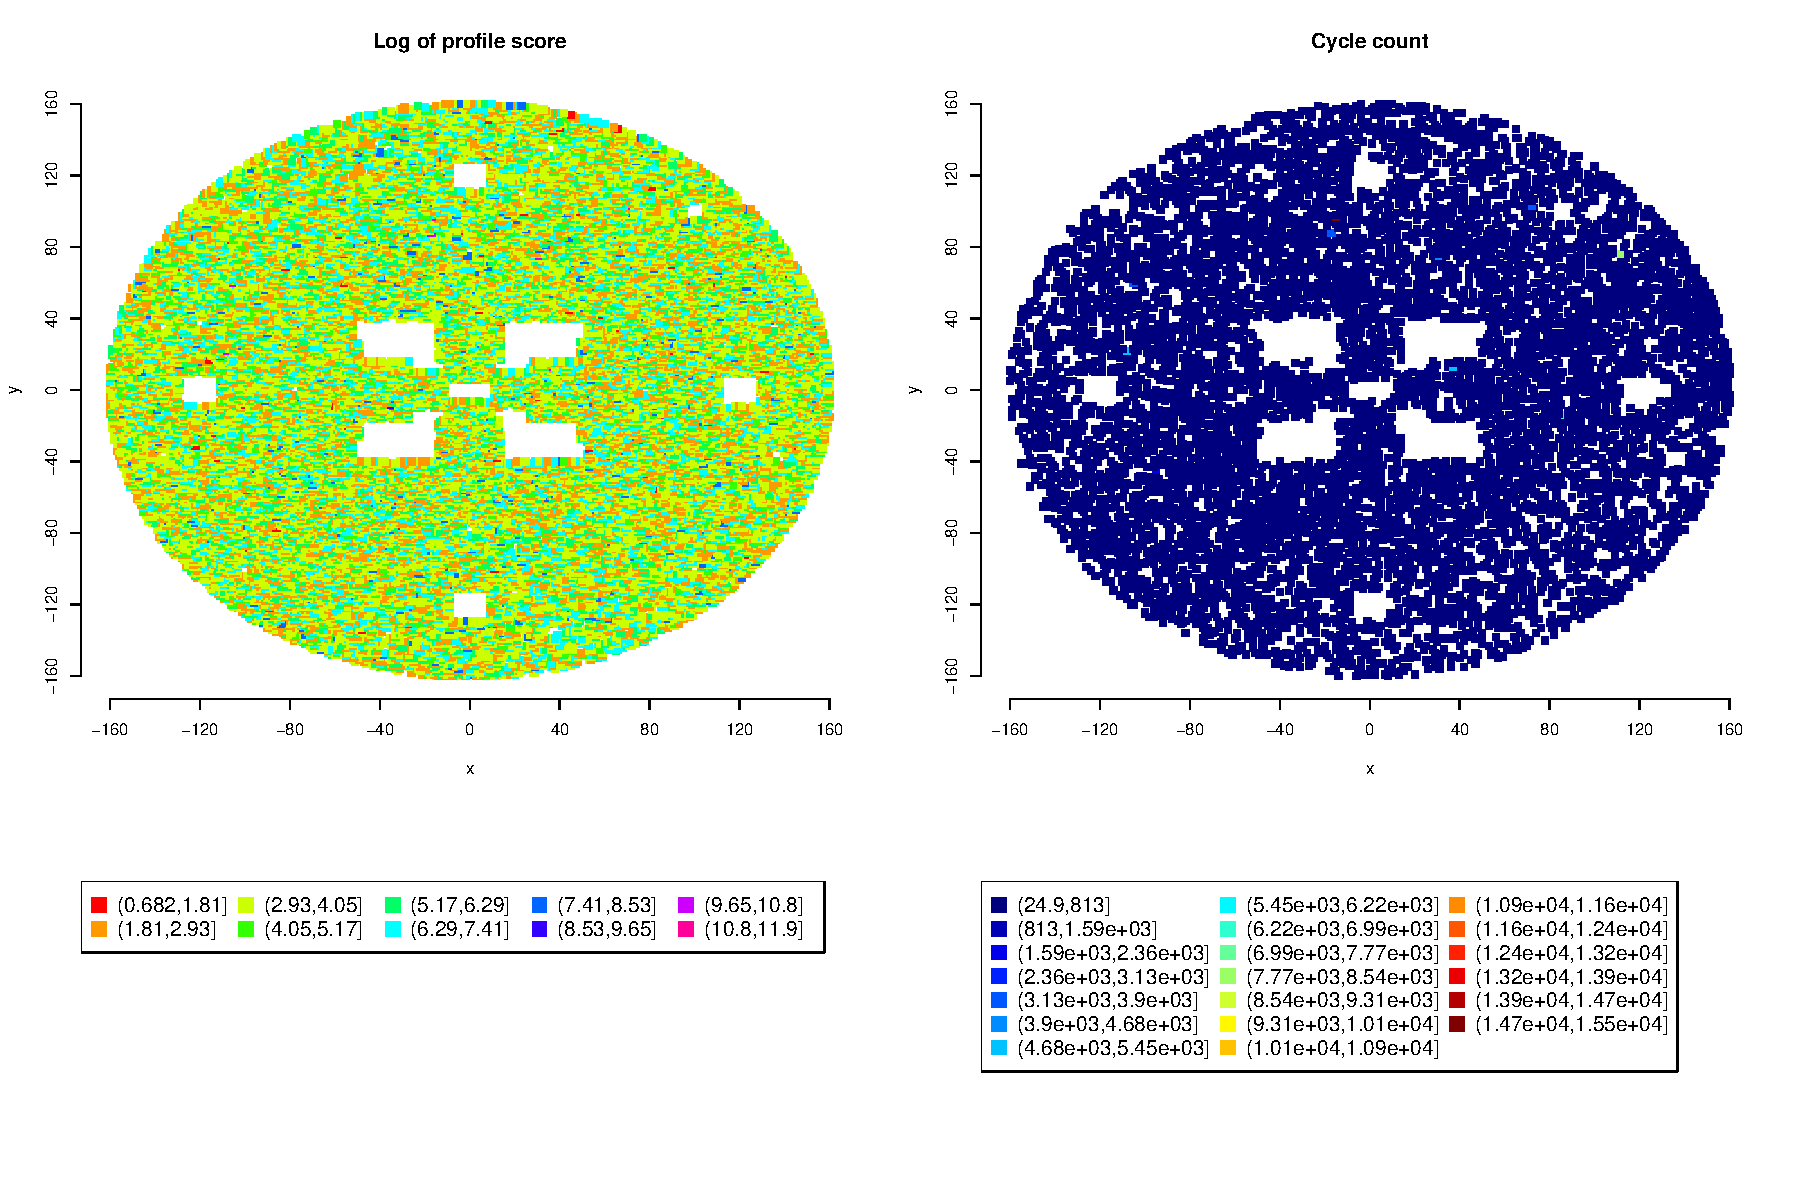
\includegraphics[width=\maxwidth]{figure/unnamed-chunk-6-1} 

\end{knitrout}
\begin{scriptsize}
\begin{landscape}
% latex table generated in R 3.2.2 by xtable 1.8-0 package
% Mon Aug 29 13:13:04 2016
\begin{table}[ht]
\centering
\begin{tabular}{rrrrrrrrrrrrrr}
  \hline
 & hole.number & x & y & subreads & avg.seq.len & HQ.region.len & avg.score & min.cycle & avg.cycle & max.cycle & min.regex & avg.regex & max.regex \\ 
  \hline
1 & 91357 & -15 &  97 &   1 & 58297.00 & 58297 & 145800.00 & 10000 & 15492.00 & 15492 & 10000 & 15843.00 & 15843 \\ 
  2 & 16165 & 111 &  76 &   1 & 27558.00 & 27558 & 69396.00 & 7862 & 7862.00 & 7862 &  12 & 12.00 &  12 \\ 
  3 & 28528 &  87 & -14 &   1 & 26413.00 & 26413 & 55106.00 & 6797 & 6797.00 & 6797 &  77 & 77.00 &  77 \\ 
  4 & 57902 &  37 &  13 &   1 & 20632.00 & 20632 & 39680.00 & 5241 & 5241.00 & 5241 &  81 & 81.00 &  81 \\ 
  5 & 145755 & -108 &  22 &   1 & 24858.00 & 24858 & 27446.00 & 5126 & 5126.00 & 5126 & 138 & 138.00 & 138 \\ 
  6 & 62070 &  31 &  75 &   1 & 24979.00 & 24979 & 15786.00 & 4379 & 4379.00 & 4379 & 199 & 199.00 & 199 \\ 
  7 & 37074 &  72 & 103 &   1 & 17042.00 & 17042 & 29074.00 & 3902 & 3902.00 & 3902 &  78 & 78.00 &  78 \\ 
  8 & 144583 & -105 &  60 &   1 & 15433.00 & 15433 & 30524.00 & 3728 & 3728.00 & 3728 & 3700 & 3700.00 & 3700 \\ 
  9 & 92632 & -17 &  88 &   1 & 12809.00 & 12809 & 24708.00 & 3248 & 3248.00 & 3248 &  32 & 32.00 &  32 \\ 
  10 & 139162 & -95 & -44 &   1 & 11247.00 & 11247 & 6692.00 & 2045 & 2045.00 & 2045 & 100 & 100.00 & 100 \\ 
  11 & 104324 & -35 &  -8 &   1 & 2852.00 & 2852 & 5394.00 & 720 & 720.00 & 720 &   8 & 8.00 &   8 \\ 
  12 & 81885 &   0 & -17 &   1 & 4717.00 & 4717 & 2698.00 & 638 & 638.00 & 638 & 607 & 607.00 & 607 \\ 
  13 & 108346 & -42 & -63 &   2 & 6839.50 & 13727 & 2878.00 & 281 & 501.50 & 722 & 164 & 399.50 & 635 \\ 
  14 & 16745 & 110 & -52 &   1 & 3427.00 & 3427 & 2742.00 & 496 & 496.00 & 496 & 520 & 520.00 & 520 \\ 
  15 & 113348 & -50 & -15 &   1 & 3605.00 & 3605 & 1989.00 & 492 & 492.00 & 492 & 494 & 494.00 & 494 \\ 
  16 & 27872 &  88 & -128 &   1 & 3762.00 & 3762 & 2148.00 & 459 & 459.00 & 459 & 487 & 487.00 & 487 \\ 
  17 & 102180 & -32 &  60 &   1 & 3391.00 & 3391 & 3198.00 & 451 & 451.00 & 451 & 454 & 454.00 & 454 \\ 
  18 & 16942 & 109 & -92 &   1 & 3049.00 & 3049 & 1786.00 & 427 & 427.00 & 427 & 437 & 437.00 & 437 \\ 
  19 & 73635 &  13 & 130 &   1 & 3593.00 & 3593 & 1323.00 & 420 & 420.00 & 420 & 416 & 416.00 & 416 \\ 
  20 & 125707 & -70 &  65 &   1 & 4765.00 & 4765 & 1864.00 & 402 & 402.00 & 402 & 388 & 388.00 & 388 \\ 
  21 & 46389 &  56 & -67 &   1 & 2234.00 & 2234 & 1974.00 & 400 & 400.00 & 400 & 379 & 379.00 & 379 \\ 
  22 & 47210 &  55 & 148 &   1 & 3154.00 & 3154 & 2114.00 & 399 & 399.00 & 399 & 403 & 403.00 & 403 \\ 
  23 & 16415 & 111 &  91 &   1 & 4364.00 & 4364 & 940.00 & 396 & 396.00 & 396 &  31 & 31.00 &  31 \\ 
  24 & 89461 & -12 & 130 &   1 & 3259.00 & 3259 & 2796.00 & 395 & 395.00 & 395 & 403 & 403.00 & 403 \\ 
  25 & 149039 & -115 &  30 &   1 & 2917.00 & 2917 & 1534.00 & 395 & 395.00 & 395 & 393 & 393.00 & 393 \\ 
  26 & 50855 &  49 & 123 &   1 & 2081.00 & 2081 & 2288.00 & 384 & 384.00 & 384 &  15 & 15.00 &  15 \\ 
  27 & 158331 & -138 & -33 &   1 & 2482.00 & 2482 & 2258.00 & 377 & 377.00 & 377 & 386 & 386.00 & 386 \\ 
  28 & 79137 &   4 & 142 &   1 & 3470.00 & 3470 & 1684.00 & 375 & 375.00 & 375 & 399 & 399.00 & 399 \\ 
  29 & 159528 & -142 &  42 &   1 & 2440.00 & 2440 & 2082.00 & 368 & 368.00 & 368 & 369 & 369.00 & 369 \\ 
  30 & 126954 & -73 & -133 &   1 & 2154.00 & 2154 & 2394.00 & 359 & 359.00 & 359 & 368 & 368.00 & 368 \\ 
  31 & 158681 & -139 & -11 &   1 & 4196.00 & 4196 & 1676.00 & 353 & 353.00 & 353 & 351 & 351.00 & 351 \\ 
  32 & 96246 & -23 & -145 &   1 & 3460.00 & 3460 & 1288.00 & 352 & 352.00 & 352 & 362 & 362.00 & 362 \\ 
  33 & 88936 & -11 & -72 &   1 & 3213.00 & 3213 & 1996.00 & 346 & 346.00 & 346 & 384 & 384.00 & 384 \\ 
  34 & 130611 & -79 & 107 &   1 & 3219.00 & 3219 & 1998.00 & 343 & 343.00 & 343 & 395 & 395.00 & 395 \\ 
  35 & 141356 & -99 &  85 &   1 & 2181.00 & 2181 & 1756.00 & 341 & 341.00 & 341 & 313 & 313.00 & 313 \\ 
  36 & 131073 & -80 &   7 &   1 & 2197.00 & 2197 & 1236.00 & 332 & 332.00 & 332 & 314 & 314.00 & 314 \\ 
  37 & 17043 & 109 &   9 &   1 & 2198.00 & 2198 & 2334.00 & 331 & 331.00 & 331 & 362 & 362.00 & 362 \\ 
  38 & 74721 &  11 & -75 &   1 & 2998.00 & 2998 & 1182.00 & 328 & 328.00 & 328 & 347 & 347.00 & 347 \\ 
  39 & 81633 &   0 &  54 &   1 & 4932.00 & 4932 & 1098.00 & 328 & 328.00 & 328 & 340 & 340.00 & 340 \\ 
  40 & 42419 &  62 & -128 &   1 & 3031.00 & 3031 & 1938.00 & 325 & 325.00 & 325 &  44 & 44.00 &  44 \\ 
   \hline
\end{tabular}
\end{table}

\end{landscape}
\end{scriptsize}

\section{Future}
\begin{enumerate}
  \item At the moment we lack the pulse data files, but ...
  \item Analysis of neighboring holes and their effect to the center ?
  \item 
  
\end{enumerate}

\end{document}
